\bartchapterimage{sdss}
\bartthumb{thumb_sdss}
\chapter{Analysing SDSS-DR8\label{ap:sdss}}
%
\section{Introduction}
%
%
\section{Analysis}
%
\subsection{Definitions}
%
Strips are bands of observations along great circles of the survey. Each of
them is composed of six parallel scanlines (of 13 arcmin wide) with gaps of
approximately the same width between the between them. Two strips make a
single stripe of 2.5°. Each scanline include all the data (in $ugriz$), and
is divided in fields (which can overlap). So when accessing to an
observation at a given position in the sky, we access a specific field. A
given observation is completely defined by its run number, the number of the
camcol of the scanline and by the field number.

On each field, the pipeline of the SDSS is applied for the objects
extraction. They are detected as pixels over-densities relatively to the
background. With this method, multiple real and different objects can be
seen as one. They are linked by their pixels as galaxies in
Friends-of-Friends algorithm. A deblending algorithm is then applied to
resolve child objects from their parents (defined as the first detection).
Then a resolve algorithm is applied to extract the best object when multiple
fields are overlapping.

Flags exist for selection with good galaxies. For example, \texttt{FLAGS1}
and \texttt{FLAGS2} flags are combined in a 64 bits mask \texttt{FLAGS} to
know bad object with poor photometry. In the \texttt{Photometry} table,
there is also a \texttt{clean} for a predefined selection of the most common
good flags, and facilitate the selection.

There is many problems with photometry, with cases of bright galaxies with
sky levels not well estimated and missing faint galaxies for example. Most
of these known problems are corrected in the recent releases (DR9 and DR10).

Old releases worked with a spectrograph of 640 fibers, with collisions at
55'', while the new BOSS survey works with a 1000 fibers spectrograph but
with a greater collision size of 64''. The coverage of the old releases
should be used for the new BOSS, so its better to use latest releases.
Moreover, the pipeline used for the spectrum had changed and improved along
releases.

Following definitions given in the SDSS website, we can define two
coordinate systems in the survey.
%
\begin{description}
    \item[Great Circle:] This coordinates system is define with two angles
        $(\mu, \nu)$. Coordinates are relatives to one stripe so they can be
        used when working with galaxies inside a stripe region.

    \item[Survey Coordinates:] It's an other system similar to celestial
        coordinates but ``centred'' on the contiguous block of galaxies  of
        the survey. Coordinates are written $(\lambda, \eta)$. The range of
        these coordinates is: $-\cfrac{\pi}{2}<\eta<\cfrac{\pi}{2}$ and
        $-\pi<\lambda<\pi$.
\end{description}
%
We will work only with survey coordinates as they allow us to easily define
a mask for the SDSS\@. The celestial coordinates and survey coordinates are
the same system of coordinates, except that one is a particular rotation of
the other. The relation between the two systems can be computed and are:
%
\subsubsection{Survey coordinates to celestial coordinates}
%
\begin{eqnarray}
    \delta &=& \arcsin\left(\cos\lambda\sin\left(\eta+\delta_0\right)\right)\nonumber\\
    \alpha &=&
    \mathrm{atan2}\left(\sin\lambda,\cos\lambda\cos\left(\eta+\delta_0\right)\right)+\lambda_0\nonumber\\
\end{eqnarray}
%
with
${(\alpha_0,\delta_0)}_{(\alpha,\delta)}={(185°,32.5°)}_{(\alpha,\delta)}={(0,0)}_{(\lambda),
\eta}$.
%
\subsubsection{Celestial coordinates to survey coordinates}
%
The inverse transformation is:
%
\begin{eqnarray}
    \eta &=& \mathrm{atan2}\left(\sin\delta,\cos\delta\cos\left(\alpha-\alpha_0\right)\right)-\delta_0\nonumber\\
    \lambda &=& \arcsin\left(\cos\delta\sin\left(\alpha-\alpha_0\right)\right)\nonumber\\
\end{eqnarray}
%
with
${(\alpha_0,\delta_0)}_{(\alpha,\delta)}={(185°,32.5°)}_{(\alpha,\delta)}={(0,0)}_{(\lambda),
\eta}$. Periodic conditions must be applied to angles found by the latter
equation:
%
\begin{equation}
    \begin{cases}
        \eta\rightarrow\eta+180° \; \lambda\rightarrow180°-\lambda&
        \mbox{if} \eta<-90°\;\mbox{or}\; \eta>90°\\
        \eta\rightarrow\eta-360° &
        \mbox{if} \eta>180°\\
        \lambda\rightarrow\lambda-360° &
        \mbox{if} \lambda>180°\\
    \end{cases}
\end{equation}
%
\subsubsection{Stripe number}
%
Stripes have a constant width of 2.5° along the $\eta$ coordinate, with a
width of 2.5°. So, stripe number $n$ of a galaxy with $\eta$ coordinate is:
%
\begin{equation}
    n = \mathrm{floor}\left(\cfrac{\left(\eta+58.75°\right)}{2.5°}\right)
\end{equation}
%
\subsection{Galaxies selection}
%
Many tables in the SDSS save galaxies and other objects properties extracted
from images of the survey. These tables are the results of different
selections in objects extracted in images. When crossing objects between
images of the survey that overlap, there are some differences of positions
between the same object in the two images. So there are possibilities that
an object is observed twice or more. In many of those tables, there is no
object duplicated.

In the SDSS database, the \texttt{Galaxy} view is a selection from the
\texttt{PhotoPrimary} for objects flagged as \emph{galaxy}. The
\texttt{Galaxy} view contains the photometric parameters (no redshifts or
spectroscopic parameters) measured for resolved primary objects. But we have
other useful informations to link with tables that give us photometric and
spectroscopic redshifts. There is the \texttt{specobjid} to link with
spectroscopic redshifts in the table \texttt{SpecObj} which doesn't contain
duplicates (it's a clean table of \texttt{SpecObjAll} with clean redshifts).
If \texttt{specobjid=0}, the galaxy doesn't have a spectroscopic redshift
(the galaxy wasn't spectroscoped). The \texttt{objid} is a link to the
\texttt{Photoz} table which contains all photometric redshifts for galaxies
in the \texttt{Galaxy} table. Estimation is based on a robust fit on
spectroscopically observed objects with similar colors and inclination
angle. There is also the \texttt{PhotozRF} where estimates are based on the
Random Forest technique. Galaxies in the \texttt{SpecObj} are limited to
$m_r<17.77$ and a given surface brightness. So we need to apply the same
flux limitations when selecting galaxies on the \texttt{Galaxy} table. A
possible \texttt{SQL} query for selecting galaxies in this table and link
them with redshift tables is for spectroscoped galaxies:
%
\begin{listing}[H]
    \begin{minted}[bgcolor=griscode, linenos]{sql}
SELECT GG.ra, GG.dec, GG.petroMag_u, GG.petroMag_g, GG.petroMag_r,
GG.petroMag_i, GG.petroMag_z, GG.specobjid, GG.objid, Z.z, Z.Zerr
FROM Galaxy AS GG, SpecObj AS Z WHERE Z.specobjid=GG.specobjid AND
GG.specobjid!=0 AND GG.petroMag_r<17.77 AND GG.ra<275 AND GG.ra>100 AND
GG.dec>-10 AND GG.dec<75
    \end{minted}
\end{listing}
%
and for galaxies which couldn't be spectroscoped:
%
\begin{listing}[H]
    \begin{minted}[bgcolor=griscode, linenos]{sql}
SELECT GG.ra, GG.dec, GG.petroMag_u, GG.petroMag_g, GG.petroMag_r,
GG.petroMag_i, GG.petroMag_z, GG.specobjid, GG.objid, Z.z, Z.Zerr
FROM Galaxy AS GG, Photoz AS Z WHERE GG.specobjid=0
AND GG.objid=Z.objid AND GG.petroMag_r<17.77 AND GG.ra<275
AND GG.ra>100 AND GG.dec>-10 AND GG.dec<75
    \end{minted}
\end{listing}

Stripe limits are given in the table \texttt{StripeDefs} but this
limits aren't actual, they were planned at the beginning of the survey.

Some planned regions aren't still observed, so we need to define other
limits in $\lambda$ coordinates for not complete stripes. We find by hand
the new limits of stripes which contains spectroscoped galaxies. Now, the
survey mask is like in figure (\ref{fig:sdss}). We will
consider just galaxies in this mask in order to find groups in the SDSS\@.
%
\begin{figure}[ht]
    \centering
    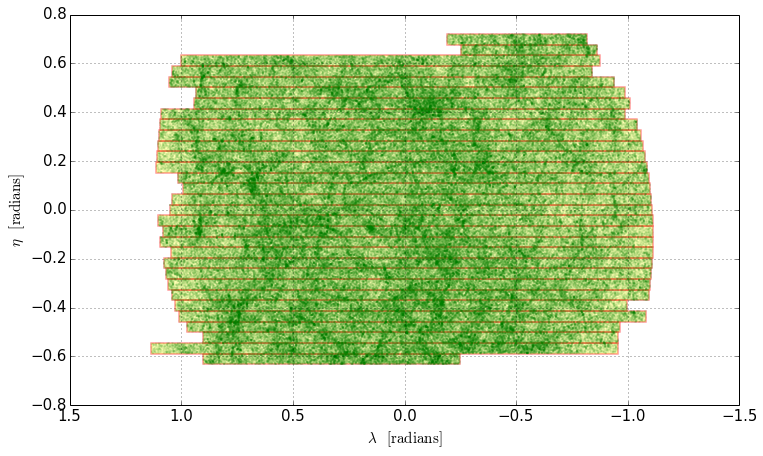
\includegraphics[width=\linewidth]{figures/sdss/sdss.png}
    \caption{Galaxies in the SDSS DR10 with stripes limits defined by hand.
    The red lines limits of the stripes make the SDSS mask used to identify
edges.\label{fig:sdss}}
\end{figure}
%
\subsubsection{Flags in the SDSS}
%
Galaxy photometry can have some troubles in the SDSS\@. In the general case,
those objects are flagged with the \texttt{clean} property which indicates
by 1 that the photometry is OK and by 0 when there is a problem. Details of
the problems are in the bit flag. But for groups, we need to select all
galaxies, even if they are not clean, or our groups will suffer
incompleteness in their members and their physical properties such as
luminosity, stellar mass\ldots will be biased.

\texttt{Galaxy} table is a selection from \texttt{PhotoPrimary} view for
objects with $\mathrm{\texttt{type}}=3$ (galaxy).
\com{%
    I think that we don't have to care of the ``good'' photometry of
    galaxies in the \texttt{Galaxy} view, but we can leave a flag in the
    group finder algorithm to say if a galaxy is in this case.
}

However, we have to take into account the error on the redshift estimation
using the \texttt{zErr}. For photometric redshift, if the \texttt{zErr} is
too high, we can use the \texttt{nnAvgZ} which is the average redshift of
galaxies in the neighbourhood of the considered galaxy. It can be better too
if the photometric redshift is too different from it.

The \texttt{SpecObjAll} contains duplicates and bad datas. But the
\texttt{SpecObj} contains just clean spectras. The field \texttt{zWarning}
can be used to decide if we keep a redshift or not.
%
\subsection{Fibre collision estimation}
%
We need a sample of galaxies for which we can easily characterize borders
and where all galaxies, given the flux limit of the survey, are presents.
But there is the problem of fibre collisions galaxies But our algorithm is
tested on a ``perfect'' mock catalogue. In order to know the behaviour of
the algorithm with these problematic galaxies, we need to implement this in
our mock catalogue.

In the SDSS, obtaining spectroscopic redshifts of galaxies is done using a
plate of 1.5° diameter, in which there is a certain number of fibres in
order to get spectrum of the galaxy. But in the plate, the number of fibres
is limited. Moreover, each portion of the sky can't be respectroscoped
multiple times, because spectrum are acquired slowly. Although runs may
overlap, there are galaxies that can't be spectroscoped. Indeed, fibres have
a dimension of 55''. When galaxies are closer than this distance, one (or
more) of those galaxies aren't spectroscoped. We can see that in the figure
(\ref{fig:plane}) where we have taken the nearest neighbour of a galaxy
on the celestial sphere, and determined the differences in angular size and
redshift between the two galaxies. As expected, the number of galaxies which
are closer than 55'' decreases dramatically. There are still some galaxies
because the overlapping of runs can permit to get redshifts for galaxies
behind this limit.
%
\begin{figure}[ht]
    \centering
    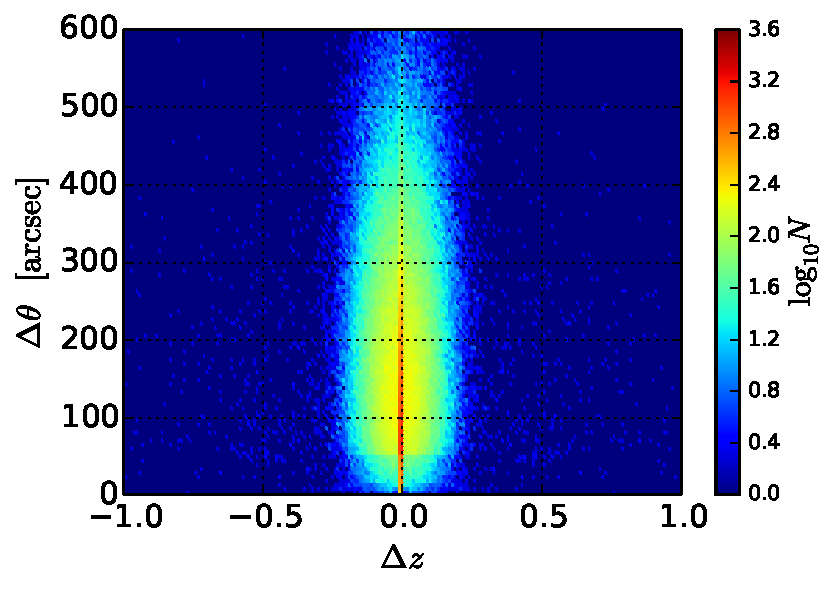
\includegraphics[width=0.6\linewidth]{figures/sdss/plane.pdf}
    \caption{\footnotesize{}Distribution of spectroscoped galaxies in the
    SDSS DR8 in angular size and redshift differences with the nearest
neighbour galaxy.\label{fig:plane}}
\end{figure}
%
A consequence is that in denser regions, the number of fibre collision
increases, affecting more our groups analysis.

We tried to implement this selection effect in our mock catalogue. For that
we computed the local density in the field, taking all galaxies
(spectroscoped or not) in the neighbourhood of 1.5° of each galaxy, and in
the same time, we determine the fraction of galaxies that don't have a
spectroscopic redshift. We expected to deduce a relation between the density
field and the fraction of fibre collisions. In the mock catalogue, we will
compute the same density field and we apply the relation estimated in the
SDSS sample to the mock. We need for each galaxy to count the fraction of
non spectroscoped galaxies in a region of 1.5° radius around. We have to
remove galaxies that are close to survey edges, because if we don't, there
are missing galaxies and the fraction will be affected. The way of selecting
those galaxies is to compute a circle of 1.5° around a galaxy, and if a
generated point is out of the survey, the galaxy is defined as to be closer
to the limits.

\remark{%
    We can generate samples of points at an angular distance $d$ to a point
    of coordinate $(\alpha_0,\delta_0)$ using formulas of the spherical
    triangle. If we define a triangle by the pole, the point
    $(\alpha_0,\delta_0)$ and the point whose we want coordinates
    $(\alpha,\delta)$, we can write the following relations using the
    spherical triangle and its dual:
    %
    \begin{eqnarray}
        \sin\delta&=&\sin\delta_0\cos d + \cos\delta_0\sin d
        \cot\gamma\nonumber\\
        \sin\delta_0\cos\gamma&=&\cos\delta_0\cot{d}-\sin\gamma\cot\left(\alpha-\alpha_0\right)\nonumber\\
    \end{eqnarray}
    %
    where $\gamma$ is like a polar angle, which have all the values between 0
    and $2\pi$. We can rewrite:
    %
    \begin{eqnarray}
        \delta &=&
        \arcsin\left(\sin\delta_0\cos d + \cos\delta_0\sin d\cos\gamma\right)\nonumber\\
        \alpha-\alpha_0 &=& \arctan\left(\cfrac{\sin\gamma}{\cos\delta_0\cot{d}-\sin\delta_0\cos\gamma}\right)\nonumber\\
    \end{eqnarray}
    %
    There are problems at poles. For a $\gamma_0$ limit, angles can't be recovered
    with above formulas. Indeed, the problem appears when
    $\tan\Delta\alpha\rightarrow\infty$. So:
    %
    \begin{equation}
        \cos\delta_0\cot d -\cos\gamma_0\sin\delta_0 = 0
    \end{equation}
    %
    implying:
    \begin{equation}
        \cos\gamma_0=\cfrac{1}{\tan d\tan\delta_0}
    \end{equation}
    %
    So to handle these limit cases, we summarize the correction for the
    differences in right ascensions by:
    %
    \begin{eqnarray}
        \Delta\alpha \rightarrow \Delta\alpha+\pi &\mathrm{if}&
        \mathrm{sign}\left(\delta_0\right)\cos\gamma \geqslant
        \mathrm{sign}\left(\delta_0\right)\cos\gamma_0\nonumber\\
    \end{eqnarray}
    %

    An other way to draw circles in the sphere is to consider the point for
    which we want to know celestial coordinates around a given angular
    distance as the pole of a new coordinate system. In this system, points
    at given distance of our central point are just points with
    $\pi/2-\delta$ and $\alpha$ running between 0 and $2\pi$. We now can
    determine cartesian coordinates of those points in this system and apply
    a rotation to go from the ``real'' system and the system where the
    central point is the pole. This can be easily done if we know the axis
    of rotation and the angle using quaternions, numerically better than
    Euler angles.
}
%
We didn't see the trend we expected with the density field, so we thought
that it can be due to the large area in which we compute the fraction of
spectroscoped galaxies and we ran the same with a radius of 0.3°, but
without success too.

Moreover, including photometric redshifts in the mock catalogue and in
MAGGIE is very complex. For example, we measured the bias and dispersion of
the distribution of differences between spectrocoped and photometric
redshifts in the SDSS\@. While the dispersion remains roughly constant, the
bias increases with the spectroscoped redshift. So some effects are not
still under control when computing photometric redshifts, and we should
avoid their utilization in any galaxy group algorithm.
%
\begin{figure}[htb]
    \centering
    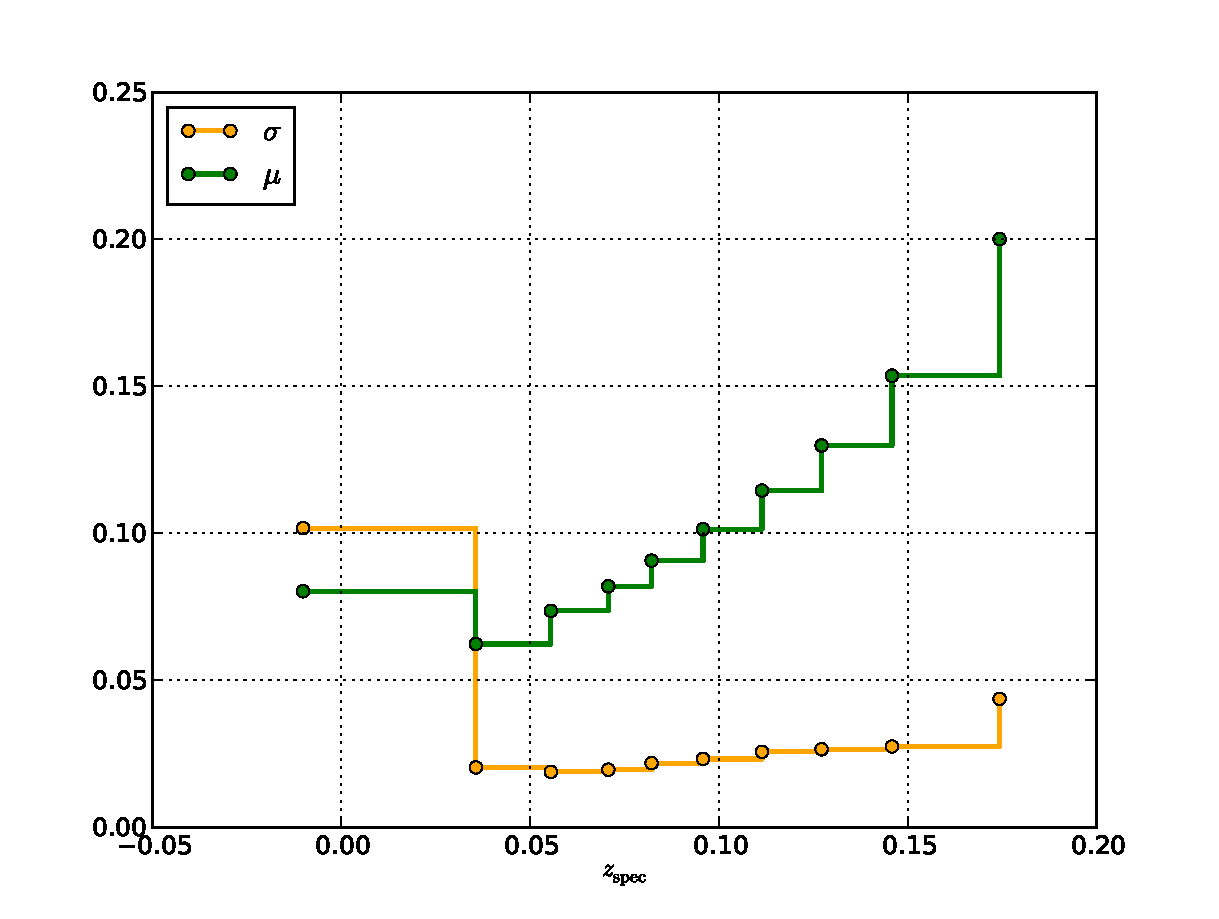
\includegraphics[width=0.8\linewidth]{figures/sdss/redshift_difference.pdf}
    \caption{Parameters of a normal distribution for photometric redshifts
    versus spectroscopic redshifts in the SDSS\@.}
\label{fig:redshift_difference}
\end{figure}
%
\note{Redo this graph}
%
\section{Coverage of the SDSS}
%
For many computations in this thesis, we need to determine the surface covered
on the sky by the galaxy sample used. In the SDSS, the mask we constructed
allows us to do it easily by a Monte Carlo process.

First, we generate a number $N$ of points around a point of coordinates
$(\alpha_0, \delta_0)$ with a maximal angular separation $\theta_{\max}$
which is larger than the maximal angular separation in our sample. The
fraction of points falling inside the mask gives us the fraction of the
generated area corresponding to the mask. This area is just
$\mathcal{S}=\int_0^{\theta_{\max}}\int_0^{2\pi}\sin\theta\dd{\theta}\dd{\phi}=
2\pi\left(1-\cos\theta_{\max}\right)$. We made this calculation for
different cone angles $\theta_{\max}$ and for different number of points to
see if we have a convergence in the value of the area. Results are shown on
figure (\ref{fig:sdss_area}).
%
\begin{figure}[htb]
    \centering
    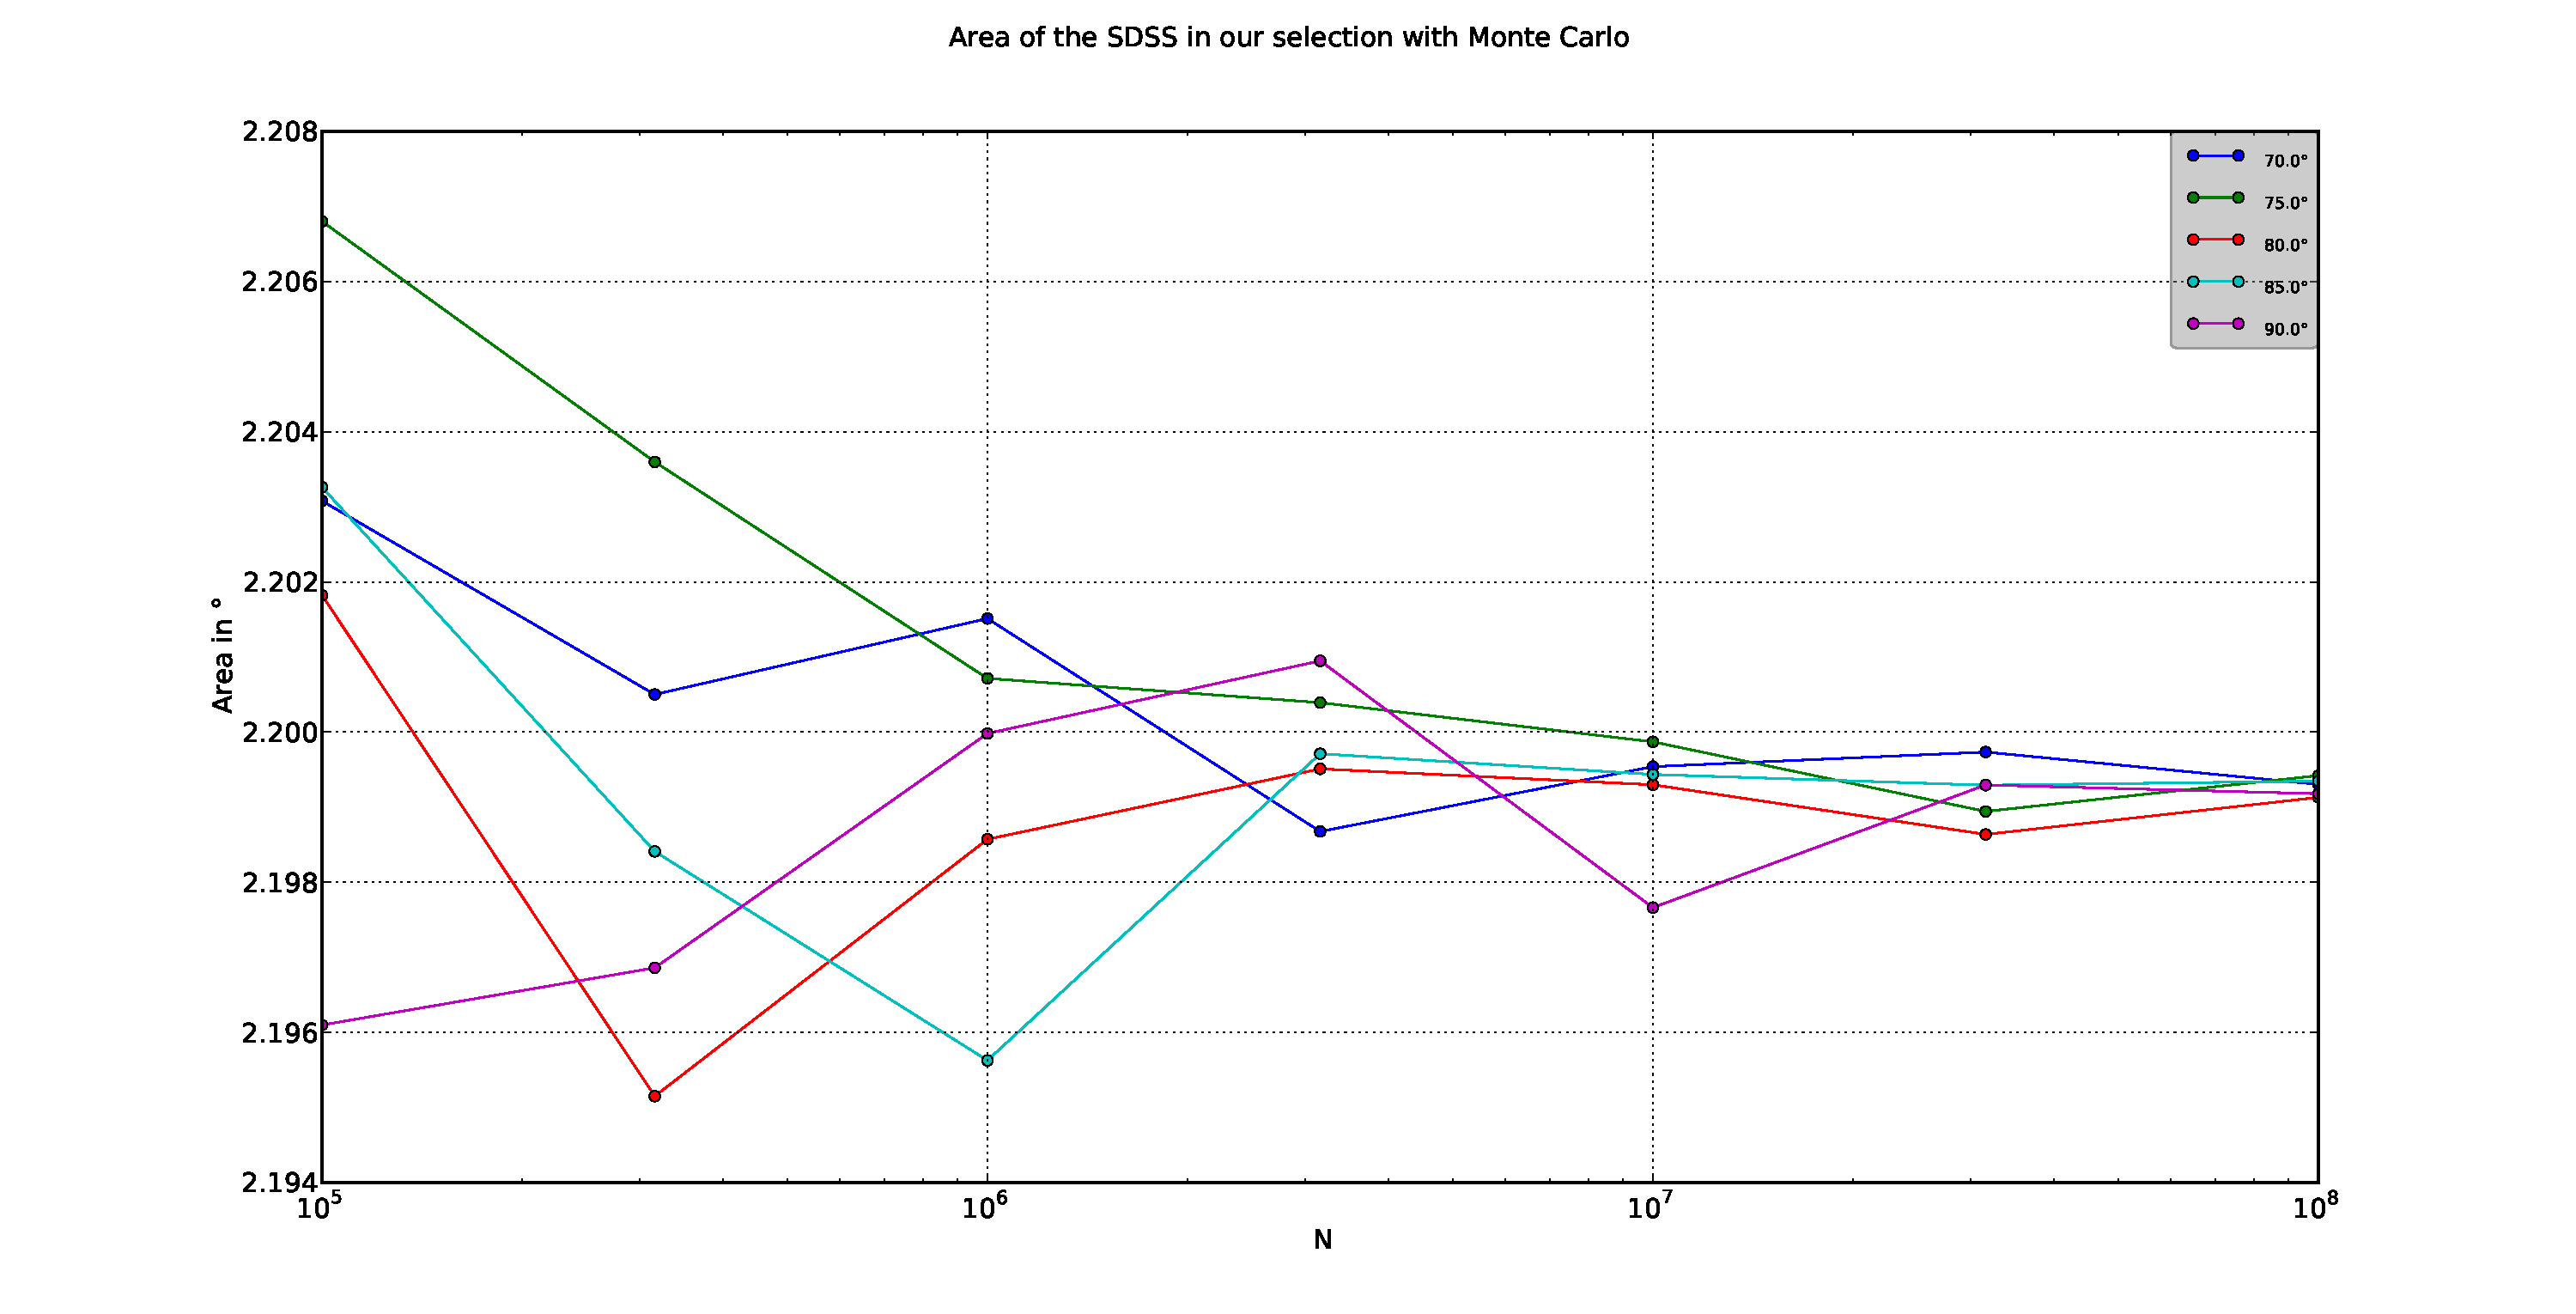
\includegraphics[width=0.8\linewidth]{figures/sdss/SDSS_area}
    \caption{Determination of the area of the SDSS for our selection with a
    Monte Carlo process. Results seem to converge on a value of 2.1993
steradians (roughly $7220°^2$).\label{fig:sdss_area}}
\end{figure}
%
\remark{%
    Generating points uniformly on the celestial sphere around a point of
    coordinates $(\alpha_0, \delta_0)$ to an angular distance $d$ can be
    done by assuming that this point is the upper pole of an other spherical
    system. In this situation, points follow $0\leqslant\theta\leqslant d$
    and $0\leqslant\phi\leqslant2\pi$, assuming spherical coordinates and
    not celestial one. $\phi$ coordinates are generated between the previous
    range. For $\theta$ coordinates, since their distribution isn't uniform
    $\left(f\left(\theta\right)=\cfrac{1}{2}\sin\theta\right)$, they are generated by
    $\theta=\arccos(2U-1)$, where $U$ is a variable following an uniform
    distribution with values between 0 and 1.

    Then, points are rotated by quaternions to $(\alpha_0, \delta_0)$. The
    rotation axis is just the cross product between the pole vector and the
    vector defined by $(\alpha_0, \delta_0)$, and the rotation angle is
    $\cfrac{\pi}{2}-\delta_0$.
}
